%%%%%%%%%%%%%%%%%%%%%%%%%%%%%%%%%%%%%%%%%
% Memo
% LaTeX Template
% Version 1.0 (30/12/13)
%
% This template has been downloaded from:
% http://www.LaTeXTemplates.com
%
% Original author:
% Rob Oakes (http://www.oak-tree.us) with modifications by:
% Vel (vel@latextemplates.com)
%
% License:
% CC BY-NC-SA 3.0 (http://creativecommons.org/licenses/by-nc-sa/3.0/)
%
%%%%%%%%%%%%%%%%%%%%%%%%%%%%%%%%%%%%%%%%%

\documentclass[letterpaper,11pt]{texMemo} % Set the paper size (letterpaper, a4paper, etc) and font size (10pt, 11pt or 12pt)

\usepackage{fancyhdr}
\usepackage{fancybox}
\usepackage{longtable}
\usepackage{amsmath}
%----------------------------------------------------------------------------------------
%	MEMO INFORMATION
%----------------------------------------------------------------------------------------



\memoto{Luis Andr\'es Valido Fajardo. luis.valido@umcc.cu (53694742)} % Recipient(s)

\memofrom{Josval Díaz Blanco} % Sender(s)

\memosubject{Guía de Aprendizaje para Concursantes ICPC y IOI: Búsqueda Binaria } % Memo subject

\memodate{\today} % Date, set to \today for automatically printing todays date

\logo{
\includegraphics[scale=0.5]{img/icpc}} % Institution logo at the top right of the memo, comment out this line for no logo

%----------------------------------------------------------------------------------------

%\titleguide{Detección de ciclos en un grafo}%cycle_graph
%\titleguide{Camino y ciclo de Hamilton}%hamilton_tour
%\titleguide{Encontrarse en el medio ( \emph{Meet in the Middle} )}%meet_in_middle
%\titleguide{Números Catalanes}%number_catalan
%\titleguide{Introducción al ajedrez}%introduction_chess 
%\titleguide{Permutaciones}%permutation FALTA
%\titleguide{Operaciones con matrices}%matrix_operation 
%\titleguide{Coeficientes binomiales}%binomial_coefficients
\titleguide{Funciones de distancias}%_distance_functions

\begin{document}

%\AddToShipoutPicture{\BackgroundPic}
\maketitle % Print the memo header information
%\tableofcontents
\pagestyle{plain}
\pagebreak

\pagestyle{fancy}
\fancyhead[LO,CE]{ }
\fancyhead[RO,CE]{
\includegraphics[scale=0.1]{img/icpc}}
\fancyfoot[LO,CE]{\textbf{Autor:} Luis Andrés Valido Fajardo \\ \textbf{Email:} luis.valido1989@gmail.com \\ \textbf{Teléfono:} 53694742}
\fancyfoot[RO,CE]{\emph{Existen 10 tipos de personas Las que \\saben binario y LAS QUE NO}}
\fancypagestyle{plain}{\pagestyle{fancy}}



%\lhead{ }
%\rhead{  }

%\fancyfoot[L]{}
%\fancyfoot[R]{\textbf{Autor:} Luis Andrés Valido Fajardo \\ \textbf{Email:} luis.valido@umcc.cu}
%----------------------------------------------------------------------------------------
%	MEMO CONTENT
%----------------------------------------------------------------------------------------


\section{Introducción}
Dentro de las áreas de conocimientos que debe conocer un competidor de programación competitiva está la geometría computacional. Dentro de los conocimientos básicos de esta área esta el poder determinar la distancia que puede existir entre dos puntos. A la diferentes funciones de distancias que debe conocer un concursantes y de como hallarla será el objetivo de la presente guía.
\section{Conocimientos previos}
\subsection{Biblioteca de funciones matemáticas}


\subsection{Funciones trigonométricas}
Las funciones trigonométricas se pueden definir como el cociente entre dos lados de un triángulo rectángulo, asociado a sus ángulos. Las funciones trigonométricas son funciones cuyos valores son extensiones del concepto de razón trigonométrica en un triángulo rectángulo trazado en una circunferencia unitaria (de radio unidad). Definiciones más modernas las describen como series infinitas o como la solución de ciertas ecuaciones diferenciales, permitiendo su extensión a valores positivos y negativos, e incluso a números complejos. 

Existen seis funciones trigonométricas básicas. Las últimas cuatro, se definen en relación de las dos primeras funciones, aunque se pueden definir geométricamente o por medio de sus relaciones. 
\section{Desarrollo}
En las matemáticas, la distancia entre dos puntos del espacio euclídeo equivale a la longitud del segmento de la recta que los une, expresado numéricamente. En espacios más complejos, como los definidos en la geometría no euclidiana, el camino más corto entre dos puntos es un segmento recto con curvatura llamada geodésica. 

\subsection{Distancia Euclidiana}
En matemáticas, la distancia euclidiana o euclídea, es la distancia ordinaria entre dos puntos de un espacio euclídeo, la cual se deduce a partir del teorema de Pitágoras. 

Esta función de distancia define la distancia entre dos puntos. La función de distancia habitual es la distancia euclidiana donde la distancia entre los puntos $(x_1, y_1)$ y $(x_2, y_2)$ es:

$$\sqrt{(x_2-x_1)^2 + (y_2-y_1)^2}$$

En general, la distancia euclidiana entre los puntos $P=(p_1,p_2,\dots,p_n)$ y 
$Q=(q_1,q_2,\dots ,q_n)$, del espacio euclídeo n-dimensional, se define como: 

$$d_E(P,Q)=\sqrt{(p_1-q_1)^2 + (p_2-q_2)^2 + \cdots + (p_n-q_n)^2} = \sqrt{\sum_{i=1}^n (p_i-q_i)^2}$$

\subsection{Distancia Manhattan}
La geometría del taxista, considerada por Hermann Minkowski en el siglo XIX, es una forma de geometría en la que la métrica usual de la geometría euclidiana es reemplazada por una nueva métrica en la que la distancia entre dos puntos es la suma de las diferencias (absolutas) de sus coordenadas. La métrica del taxista (en inglés se denomina geometría Taxicab) también se conoce como distancia rectilínea, distancia L1 o norma $\ell$, distancia de ciudad, distancia Manhattan, o longitud Manhattan, con las correspondientes variaciones en el nombre de la geometría. El último nombre alude al diseño en cuadrícula de la mayoría de las calles de la isla de Manhattan, lo que causa que el camino más corto que un auto puede tomar entre dos puntos de la ciudad tengan la misma distancia que dos puntos en la geometría del taxista. 


Una función de distancia alternativa es la distancia de Manhattan donde es la distancia entre los puntos ($x_1, y_1$) y ($x_2, y_2$) es:

$$|x_1-x_2| + |y_1-y_2|$$


\subsection{Distancia esférica}
Las personas usan latitudes (las líneas horizontales) y las longitudes (las líneas verticales) en el sistema de coordenadas de la Tierra. La longitud avanza en intervalos desde $0$ grados (Greenwich) hasta $+180^0$ * hacia el este y $-180^0$ * hacia el oeste. La latitud avanza en intervalos desde 0 grados (el Ecuador) para $+90^0$ * (hacia el Polo Norte) y $-90^0$ * (hacia el Polo Sur). 

La pregunta más interesante es: cual es la distancia / geográfica esférica entre  dos ciudades ($p$ y $q$) en tierra con radio $r$, denotada de por ($p_{lat}$,$p_{long}$) y ($q_{lat}$,$q_{long}$). Todas las coordenadas están en radianes. (o sea el rango del $-180 \dots 180$ del converso de longitud y $-90 \dots 90$ se extienden de latitudes para $-\Pi  \dots \Pi$ y $-\frac{\Pi}{2}  \dots \frac{\Pi}{2}$ respectivamente.

La fórmula de distancia esférica utiliza la fórmula del coseno para calcular la distancia entre dos puntos en la superficie esférica, teniendo en cuenta la curvatura de la esfera. Esta fórmula tiene en cuenta las coordenadas geográficas de los dos puntos, es decir, sus latitudes y longitudes en radianes.

La fórmula del coseno utiliza la función arcocoseno para calcular la distancia esférica entre los dos puntos, teniendo en cuenta la diferencia en las latitudes y longitudes de los puntos. La fórmula tiene en cuenta la curvatura de la esfera al calcular la distancia entre los dos puntos, lo que la hace más precisa que simplemente usar la distancia euclidiana en un plano. Sea una esfera sólida de centro $O$ y radio $r$ como se muestra en la figura siguiente: 

% TODO: \usepackage{graphicx} required
\begin{figure}[h!]
	\centering
	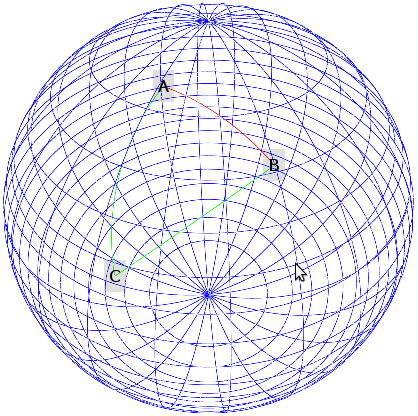
\includegraphics[width=0.3\linewidth]{img/esfera}
	\label{fig:esfera}
\end{figure}

y dos puntos $A=(x_0;y_0)$ y $B=(x_1;y_1)$ localizados sobre la superficie de la esfera, donde $x_i$, $y_i$ son coordenadas esféricas definidas como las amplitudes de los ángulos de longitud y latitud respectivamente. 

Sea la esfera de centro en el origen de coordenadas $O$ y radio $r$ y dos puntos superficiales Punto $A=(\alpha_A;\beta_A)$ y Punto $B=(\alpha_B;\beta_B)$ donde $ \alpha_A,\alpha_B \in [-\pi,\pi]$ son las longitudes de sus respectivos puntos respecto al eje x;$ \beta_A,\beta_B \in [-\frac{\pi}{2},\frac{\pi}{2}]$ son las latitudes correspondientes de $A$ y $B$. 

Traducidos a coordenadas euclideanas en el espacio los puntos $A=(x_A;y_A;z_A)=(r\cdot \cos \alpha_A \cdot \cos \beta_A; r \cdot \sin \beta_A; r \cdot \sin \alpha_A \cdot \cos \beta_A)$  y $B=(x_B;y_B;z_B)=(r\cdot \cos \alpha_B \cdot \cos \beta_B; r \cdot \sin \beta_B; r \cdot \sin \alpha_B \cdot \cos \beta_B)$ ; puede calcularse la longitud de la cuerda relativa a la ortodrómica que ambos conforman: 

$$d(A,B) = \sqrt{(B_x-A_x)^2+(B_y-A_y)^2+(B_z-A_z)^2} $$

Luego la amplitud del arco correspondiente a ese segmento es: 

$$\angle AOB = \arccos(\frac{2 \cdot r^2 - d(A,B)^2}{2 \cdot r^2})$$

Asumiendo que la función arcoseno devuelve la amplitud del ángulo en radianes. Uniendo todo, la expresión completa de la distancia esférica entre dos puntos dadas sus coordenadas esféricas queda: 

$$d_s(A,B,r) = \angle AOB \cdot r = r \cdot \arccos ( \frac{2\cdot r^2 - (x_B-x_A)^2 - (y_B-y_A)^2 - (z_B-z_A)^2}{2\cdot r^2} )$$


\section{Implementación}
\subsection{C++}
\begin{lstlisting}[language=C++]
double euclideanDistance(double x1, double y1, 
                         double x2, double y2){
   return sqrt( (x1-x2)*(x1-x2) + (y1-y2)*(y1-y2) );
}

double distanceManhattan(double x1, double y1, 
                         double x2, double y2){
   return abs(x1-x2) + abs(y1-y2);
}

//Las latitudes y longitudes de los puntos deben estar en radianes.
double distanceSpherical(double Plong, double Plat, double Qlong, 
                         double Qlat, double r){
   double Px= r* cos(Plong) * cos(Plat);
   double Py= r* sin(Plat);
   double Pz= r* sin(Plong) * cos(Plat);
   double Qx= r* cos(Qlong) * cos(Qlat);
   double Qy= r* sin(Qlat);
   double Qz= r* sin(Qlong) * cos(Qlat);
	
   double deltaXSquare = (Qx-Px)*(Qx-Px);
   double deltaYSquare = (Qy-Py)*(Qy-Py);
   double deltaZSquare = (Qz-Pz)*(Qz-Pz);
	
   double numerador = 2 * r * r - deltaXSquare - deltaYSquare - deltaZSquare;
   double denominator = 2 * r * r;
   double d = r * acos(numerador/denominator);
   return d;
}
\end{lstlisting} 

\subsection{Java}
\begin{lstlisting}[language=Java]
public static double euclideanDistance(double x1, double y1, 
                                       double x2, double y2){
   return Math.sqrt( (x1-x2)*(x1-x2) + (y1-y2)*(y1-y2) );
}
	
public static double distanceManhattan(double x1, double y1, 
                                       double x2, double y2){
   return Math.abs(x1-x2) + Math.abs(y1-y2);
}
		
//Las latitudes y longitudes de los puntos deben estar en radianes.
public static double distanceSpherical(double Plong, double Plat, 
                                       double Qlong, double Qlat, double r){
   double Px= r* Math.cos(Plong) * Math.cos(Plat);
   double Py= r* Math.sin(Plat);
   double Pz= r* Math.sin(Plong) * Math.cos(Plat);
   double Qx= r* Math.cos(Qlong) * Math.cos(Qlat);
   double Qy= r* Math.sin(Qlat);
   double Qz= r* Math.sin(Qlong) * Math.cos(Qlat);
	
   double deltaXSquare = (Qx-Px)*(Qx-Px);
   double deltaYSquare = (Qy-Py)*(Qy-Py);
   double deltaZSquare = (Qz-Pz)*(Qz-Pz);
	
   double numerador = 2 * r * r - deltaXSquare - deltaYSquare - deltaZSquare;
   double denominator = 2 * r * r;
   double d = r * acos(numerador/denominator);
   return d;
}
\end{lstlisting} 

\section{Aplicaciones}
Algunas aplicaciones de la distancia euclidiana incluyen:

\begin{enumerate}
\item \textbf{ Algoritmos de búsqueda y optimización:} La distancia euclidiana se utiliza en algoritmos de búsqueda para encontrar la ruta más corta entre dos puntos en un espacio euclidiano. También se utiliza en algoritmos de optimización para minimizar la distancia entre puntos en un espacio multidimensional.
\item \textbf{ Análisis de redes de transporte:} En el análisis de redes de transporte, la distancia euclidiana se utiliza para calcular la distancia entre nodos o puntos de interés en una red de carreteras, ferrocarriles, o rutas de transporte público.
\item \textbf{Problemas de asignación de recursos:} En problemas de asignación de recursos, la distancia euclidiana se utiliza para calcular la distancia entre diferentes ubicaciones o recursos, lo que puede ayudar a optimizar la asignación de recursos en un espacio geográfico.
\end{enumerate}

En resumen, la distancia euclidiana es una medida comúnmente utilizada en aplicaciones donde se requiere calcular distancias en un espacio euclidiano y donde los movimientos no están restringidos a movimientos verticales y horizontales, como en el caso de la distancia de Manhattan.

En el contexto de aplicaciones, la distancia de Manhattan se utiliza en diversas áreas, como en algoritmos de búsqueda y optimización, en análisis de redes de transporte y en problemas de asignación de recursos. Por ejemplo, en logística, la distancia de Manhattan puede utilizarse para calcular la distancia entre dos ubicaciones en una ciudad, considerando solo los movimientos horizontales y verticales.

En resumen, la distancia de Manhattan es una medida útil en aplicaciones donde se necesita calcular distancias en un espacio cartesiano y donde los movimientos están restringidos a movimientos verticales y horizontales.

Algunas aplicaciones de la distancia esférica incluyen:

\begin{enumerate}
	\item \textbf{Sistemas de navegación:} La distancia esférica se utiliza en sistemas de navegación para calcular la distancia entre dos puntos en la superficie de la Tierra, lo que ayuda a determinar la ruta más corta entre dos ubicaciones.
	\item \textbf{Geolocalización:} En aplicaciones de geolocalización, la distancia esférica se utiliza para calcular la distancia entre la ubicación actual de un dispositivo y puntos de interés cercanos, como restaurantes, tiendas, o eventos.
	\item \text{Astronomía:} En astronomía, la distancia esférica se utiliza para medir la distancia entre objetos celestes, como estrellas, planetas, o galaxias, que están ubicados en el espacio tridimensional.
\end{enumerate}

En resumen, la distancia esférica es una medida comúnmente utilizada en aplicaciones donde se requiere calcular distancias en la superficie de la Tierra o en el espacio tridimensional, como en el caso de la navegación, geolocalización y astronomía.

\subsection{Coordenadas giratorias}

Algunos problemas son más fáciles de resolver si se usan distancias de Manhattan en lugar de distancias euclidianas. Como ejemplo, considere un problema en el que se nos da n puntos en el plano bidimensional y nuestra tarea es calcular la distancia máxima de Manhattan entre dos puntos. Por ejemplo, considere el siguiente conjunto de puntos:

% TODO: \usepackage{graphicx} required
\begin{figure}[!h]
	\centering
	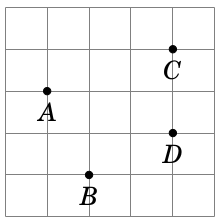
\includegraphics[width=0.25\linewidth]{img/diistance_functios_1}
	\label{fig:diistancefunctios1}
\end{figure}

La distancia máxima de Manhattan es 5 entre los puntos $B$ y $C$:

\begin{figure}[!h]
	\centering
	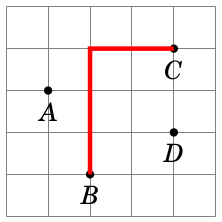
\includegraphics[width=0.25\linewidth]{img/diistance_functios_2}
	\label{fig:diistancefunctios2}
\end{figure}

Una técnica útil relacionada con las distancias de Manhattan es rotar todas las coordenadas 45 grados para que se convierta un punto $(x,y)$ a $(x + y, y - x)$. Por ejemplo, después de rotar los puntos anteriores, el resultado es:

\begin{figure}[!h]
	\centering
	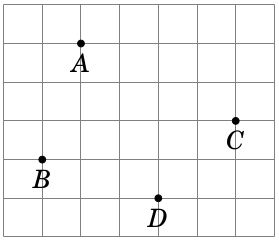
\includegraphics[width=0.25\linewidth]{img/diistance_functios_3}
	\label{fig:diistancefunctios3}
\end{figure}

Y la distancia máxima es la siguiente:

\begin{figure}[!h]
	\centering
	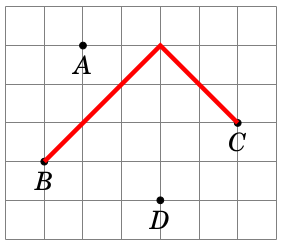
\includegraphics[width=0.25\linewidth]{img/diistance_functios_4}
	\label{fig:diistancefunctios4}
\end{figure}

Considere dos puntos $P_1 = (x_1, y_1)$ y $P_2 = (x_2, y_2)$ cuyas coordenadas rotadas son $P'_1 = (x'_1, y'_1)$ y $P'_2 = (x'_2, y'_2)$. Ahora hay dos formas de expresar la distancia de Manhattan entre $P_1$ y $P_2$:

$$|x_1-x_2|+|y_1-y_2| = \max (|x'_1-x'_2|,|y'_1-y'_2|)$$

Por ejemplo, si $P_1=(1,0)$ y $P_2=(3,3)$, las coordenadas rotadas son $P'_1=(1,-1)$ y $P'_=(6,0)$ y la distancia de Manhattan es

$$|1-3| + |0-3| = \max(|1-6|, |-1-0|) = 5$$

Las coordenadas rotadas proporcionan una forma simple de operar con distancias de Manhattan, porque podemos considerar las coordenadas X e Y por separado. Para maximizar la distancia de Manhattan entre dos puntos, debemos encontrar dos puntos cuyas coordenadas rotadas maximizan el valor de:

$$ \max (|x'_1-x'_2|,|y'_1-y'_2|) $$

Esto es fácil, porque la diferencia horizontal o vertical de las coordenadas rotadas tiene que ser máxima.


\section{Complejidad}
La complejidad de estas funciones de distnacia es bien sencilla al resultar operaciones elementales se puede definir que su complejidad es O($1$).
\section{Ejercicios}
A continuación una lista de ejercicios que se pueden resolver aplicando los contenidos abordados en la guía:

\begin{itemize}
	\item \href{https://dmoj.uclv.edu.cu/problem/claust}{DMOJ - Vacas Claustrofóbicas}
	\item \href{https://matcomgrader.com/problem/9597/colors-i/}{MOG - H - Colors I}
\end{itemize}


\end{document}